\chapter{应用层程序接口封装}
	从VxWorks6.x开始引入了RTP(VxWorks Real Time Process Project)模式,这种模式的优点是应用程序之间互相独立、互不影响,而且增加了内核的稳定性,缺点是由于“内核态”与“用户态”的内存拷贝,其执行效率有所降低,随着CPU速度越来越快,这点效率的牺牲已经越来越不重要。相比较于传统的DKM(downloadable kernel module project),RTP适合多个团队独立运作,然后汇总联试,这种模式除了全局函数不能在shell里直接调用外,其对应用程序几乎不做任何约束,原有的DKM工程代码稍作修改即可正常运行。内核变化较大,需要添加较多的组件,内存需要较好的划分,为保持应用程序直接调用函数调试的习惯,需要封装接口供用户使用。

\section{应用层接口模块设计}

	应用层的接口包括两个部分:一是标准输出重定向接口的设计,目的是在程序运行期间直接调用标准输出函数时就能够将输出信息通过我们的串口输出出去,但是这个标准输出输出的信息不是格式化的信息。二是Log接口函数,通过调用这个接口函数可以将调试信息格式化输出,输出信息会自动包括调试的级别、产生的时间、所处的文件、行号等信息,便于对调试信息进行分析。

主要的模块包块以下两个:
\begin{itemize}
\item \hei{ResetStdOut():} 提供给用户选择是否需要重定向标准输出,若参数为1则将标准输出进行重定向,若参数为0,则关闭标准输出重定向,恢复到之前的标准输出。

\item \hei{Log接口函数:} 提供封装的不同级别的Log调试接口,包括LogE(表示错误信息)、LogD(表示详情信息)、LogW(表示警告信息)、LogI(表示)
\end{itemize}

由于从VxWorks6.x开始引入了RTP(VxWorks Real Time Process Project)模式,这种模式的优点是应用程序之间互相独立、互不影响,而且增加了内核的稳定性,缺点是由于“内核态”与“用户态”的内存拷贝,其执行效率有所降低,随着CPU速度越来越快,这点效率的牺牲已经越来越不重要。在这种RTP模式下对于我们的标准输出重定向接口而言,其实现方式与task模式下存在一些差别,在task模式下我们需要使用VxWorks封装好的ioTaskStdSet()函数来实现重定向,而在RTP模式下我们无法使用,只能寻找其他的解决办法,在此处我们使用的是dup2()/dup()来实现。


\section{Log协议的设计}

对于Log接口函数我们设计为其为设计了专用的输出协议,如\autoref{fig:Log协议字段} 所示,在协议中包含了五种不同的输出级别,分别用LogE(表示错误信息)、LogD(表示调试信息)、LogW(表示警告信息)、LogI(表示详情信息)、Logo(表示其他信息)。同时我们还在协议中包含了一些调试信息所需要的关键信息字段,包括任务ID字段、任务名字段、文件名字段、行号字段、时间字段。
\begin{figure}[!h]
\centering
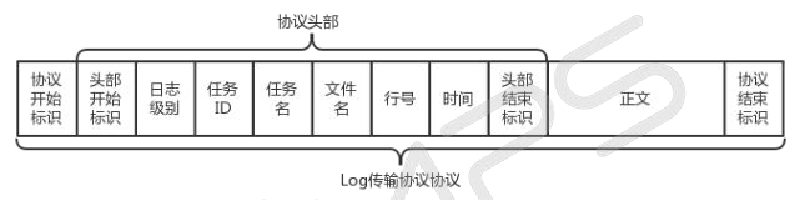
\includegraphics[width=.9\textwidth]{./graphics/Logxieyi.pdf}
\caption{Log协议字段}\label{fig:Log协议字段}
\end{figure}

我们为调试信息制定的协议格式为:\backslash 03\backslash 03<L=日志级别;PN=任务ID;P=任务名;F=文件名;N=行号;T=时间>contents\backslash 04\backslash 04\\
其中各部分的含义如下:

\begin{itemize}
\item \textbf{\backslash 03\backslash 03}:表示自定义的Log协议的数据包的开始;

\item \textbf{<}:表示自定义的Log协议数据包头部的开始;

\item \textbf{L}:表示日志的级别,我们在此将日志分为五个级别:
	\begin{itemize}
	\item e:表示error;
	
	\item w:表示warning;
	
	\item i:表示info;
	
	\item d:表示debug;
	
	\item o:表示其他信息。
	\end{itemize}
	
\item \textbf{PN}:此处的内容是输出该条调试信息的任务的任务ID;

\item \textbf{P}:此处的内容是输出该条调试信息的任务的任务名;

\item \textbf{F}:此处的内容是输出该条调试信息的任务所在的文件名;

\item \textbf{N}:此处的内容是该调试信息语句所在的文件的行号;

\item \textbf{T}:此处的内容是这条调试信息被输出时候的系统时间;

\item \textbf{>}:表示自定义的Log协议数据包头部的结束;

\item \textbf{contents}:这个部分是调试信息的正文部分。

\item \textbf{\backslash 04 \backslash 04}:表示自定义的 Log 协议数据包的结束。

\end{itemize}\\


\section{标准输出重定向接口的实现}
	由于标准输出的重定向无法在RTP模式和task模式下使用同一种方法来实现,于是我们使用了两种方法来分别实现RTP模式和task模式下的标准输出重定向。
\subsection{RTP模式下标准输出重定向}
	RTP模式下的标准输出重定向流程如\autoref{fig:rtp-printf-reset}所示。部分关键代码如下:
\lstset{language=C}
\begin{lstlisting}
int ResetStdOut(int usb_serial)
{
  ...
	
  _init_fd();
  if(usb_serial == 1)
  {
    if(dup2(log_fd,STD_OUT) < 0)
    {
      printf("can not reset STDOUT to /hust_use_serial\n");	  
	  return -1;
	}
  }
  else
  {
    if (dup2(STDOUT_FD,STD_OUT) < 0)
    {
	  printf("can not reset STDOUT to /hust_use_serial\n");
	  return -1;
	}
  }
  
  ...
}
\end{lstlisting}

\begin{figure}[!h]
\centering
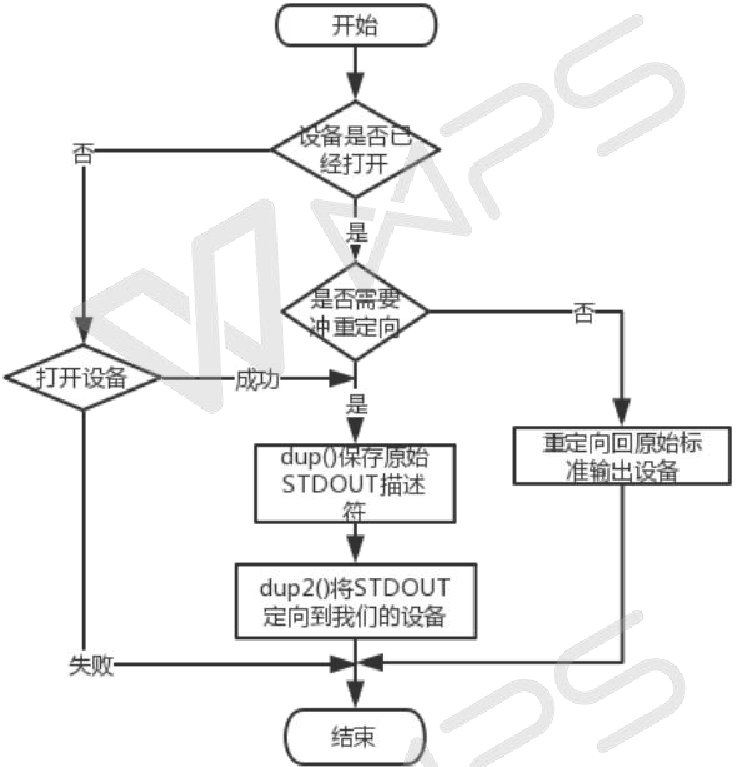
\includegraphics[width=0.7\textwidth]{./graphics/RTP-STDOUT-RESET.pdf}
\caption{RTP模式下标准输出重定向流程图}\label{fig:rtp-printf-reset}
\end{figure}


在RTP模式下使用dup2函数来实现标准输出的重定向,dup2函数的原型为:
\lstset{language=C}
\begin{lstlisting}
int dup2(int oldfd, int newfd);
\end{lstlisting}\\
dup2()用于复制描述符oldFd到newFd的,其中oldFd是要被复制的文件描述符,newFd是制定的新文件描述符,如果newFd已经打开,它将首先被关闭。如果newFd等于oldFd,dup2会返回newFd,但是不会关闭它。函数调用成功时会返回新的文件描述符,所返回的新的描述子与参数oldFd给定的描述符字引用同一个打开的文件,即共享同一个系统打开文件表项。函数调用失败时会返回-1并设置errno。

\subsection{task模式下标准输出重定向}
在task模式下无法使用dup()/dup2()函数来进行标准输出的重定向,在task模式下VxWorks有专用的标准输出接口ioTaskStdSet(),我们在此模式下只能使用这个借口来实现重定向,task模式下的标准输出重定向如\autoref{fig:task-printf-reset}所示。部分关键代码如下:
\lstset{language=C}
\begin{lstlisting}
int ResetStdOut(int usb_serial)
{
  ...
	
  _init_fd();
  if(usb_serial == 1)
  {
    ioTaskStdSet(0,STD_OUT,log_fd);
  }
  else
  {
    ioTaskStdSet(0,STD_OUT,STDOUT_FD);
  }
  
  ...
}
\end{lstlisting}

\begin{figure}[!h]
\centering
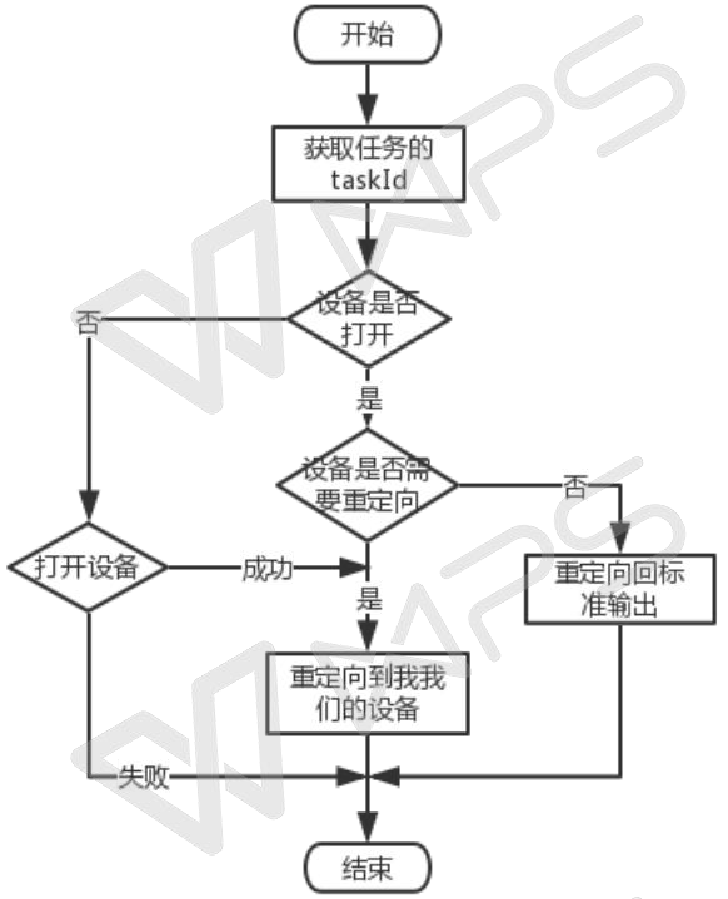
\includegraphics[width=0.7\textwidth]{./graphics/TASK-STDOUT-RESET.pdf}
\caption{task模式下标准输出重定向流程图}\label{fig:task-printf-reset}
\end{figure}

ioTaskStdSet()是VxWorks专门用来进行任务级的重定向的函数。其函数原型为:
\lstset{language=C}
\begin{lstlisting}
void ioTaskStdSet(int taskId, int stdFd, int newFd);
\end{lstlisting}\\
在VxWorks中每一个任务都有一个数组taskStd,用于表明这个任务的标准输入、标准输出、标准错误,函数ioTaskStdSet()的功能就是将特定任务的标准描述符重定向到newFd,newFd需要是一个文件或者设备的描述符。


\section{Log接口的实现}
	Log接口函数用于完成标准格式的log的输出,使用时只需要调用LogE()、LogW()、LogI()、LogD()、LogO(),这几个接口均为宏定义,定义在usb\_ logWrite.h当中,在使用时需要包含该头文件,作用是获取log协议所需要的部分信息,其代码如下所示:
\lstset{language=C}
\begin{lstlisting}
#define LogE(format, ...) usb_logWrite('e',__FILE__,__LINE__,format,##__VA_ARGS__)

#define LogD(format, ...) usb_logWrite('d',__FILE__,__LINE__,format,##__VA_ ARGS__)

#define LogI(format, ...) usb_logWrite('i',__FILE__,__LINE__,format,##__VA_ ARGS__)

#define LogW(format, ...) usb_logWrite('w',__FILE__,__LINE__,format,##__VA_ ARGS__)

#define LogO(format, ...) usb_logWrite('o',__FILE__,__LINE__,format,##__VA_ ARGS__)

extern int usb_logWrite(char level,char *fileName, int lineNum, const char * format, ...);
\end{lstlisting}
LogE(),LogW(),LogD(),LogO,LogI()均由usb\_ logWrite()函数来实现,usb\_ logWrite()函数实现真正的完整的协议封装和调用驱动发送的过程,usb\_ logWrite()完成协议头部信息的获取,包括日志的级别,发送该日志的进程号和进程名,打印该日志的文件的文件名,该日志在文件中所处的行号。并将这些信息封装在所定义的头部格式当中。最后将用户需要输出的信息放入协议的数据部分,并添加结束标志,然后调用驱动程序将该数据包发送出去。usb\_ logWrite()的部分关键代码如下所示:
\lstset{language=C}
\begin{lstlisting}
int usb_logWrite(char level,char *fileName, int lineNum, const char * format, ...)
{
  ...
   
  struct timespec tp;
  struct tm timeBuffer;
  time_t nowSec;
  char datetime[64];
  clock_gettime(CLOCK_REALTIME,&tp);
  nowSec = tp.tv_sec;
  localtime_r(&nowSec,&timeBuffer);
  timeLen = strftime(datetime,64,"%Y/%m/%d %H:%M:%S",&timeBuffer);
  sprintf(datetime+timeLen,".%3.3ld",tp.tv_nsec/1000000L);

  _init_fd();
  if(fileName != NULL) 
  {
    char *rf = strrchr(fileName, '/');
	if(rf != NULL) fileName = rf+1;
  }

  logWriteBuf[0]=0x03;
  logWriteBuf[1]=0x03;
  n = snprintf(&logWriteBuf[2],LOG_BUF_SIZE-2,"<L=%c;PN=%d;P=%s;F=%s;N=%d;T=%s>",level,Id,name,fileName,lineNum,datetime);
  n+=2;
  va_list argList;
  va_start(argList,format);
  m = vsnprintf(logWriteBuf+n,LOG_BUF_SIZE-n,format,argList);
  va_end(argList);

  if(m <= 0) 
  {
	m = snprintf(logWriteBuf+n,LOG_BUF_SIZE-n, "format error\n");
  }
  n += m;
  
  if(n > LOG_BUF_SIZE-2) n = LOG_BUF_SIZE-2;
  logWriteBuf[n++] = 0x04;
  logWriteBuf[n++] = 0x04;

  write(log_fd, logWriteBuf, n);
  return n;
}
\end{lstlisting}

usb\_ logWrite()函数的实现在RTP模式和task模式之下是一样的,在task模式下只需包含usb\_ logWrite.h头文件即可,在RTP模式下需要包含usb\_ logWrite.h和usb\_ logWrite.c两个文件。


\section{Windows下的日志分析工具}
	
	由于日志分析工具并不是我们本次论文的介绍重点,此处我们只介绍调试信息的接收部分协议的解析相关的内容,对于其他的部分不做详细介绍;日志分析工具为Windows下使用QT开发的界面程序,其结构如\autoref{fig:日志分析工具结构图}所示。
\begin{figure}[!h]
\centering
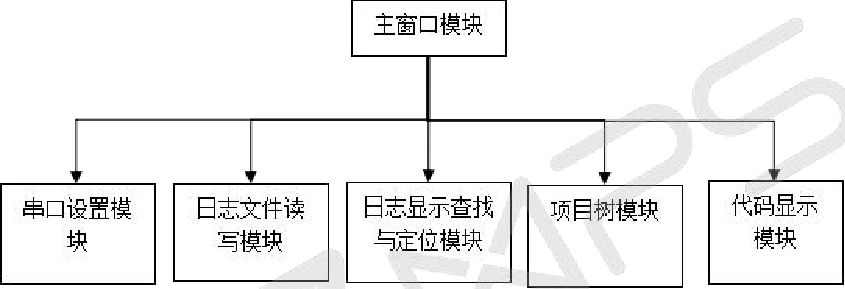
\includegraphics[width=1.0\textwidth]{./graphics/routonLog-system-structure.pdf}
\caption{日志分析工具结构图}\label{fig:日志分析工具结构图}
\end{figure}

\textbf{串口读取流程}
日志界面的串口读取流程图如\auotref{串口读取流程图} 所示,当用户打开串口后,主窗口中的串口读取函数会对串口中的数据进行非堵塞地读取,并按协议格式进行解析、显示和存盘。对于非协议格式的数据,则按照普通标准输出重定向过来的数据进行显示。此时在日志信息显示框中只会将信息显示在详细内容部分,日志级别、进程号、文件名、行号等内容均为空白。对于按照协议格式发送的信息,会按照信息的级别以不同的底色进行显示。
\begin{figure}[!h]
\centering
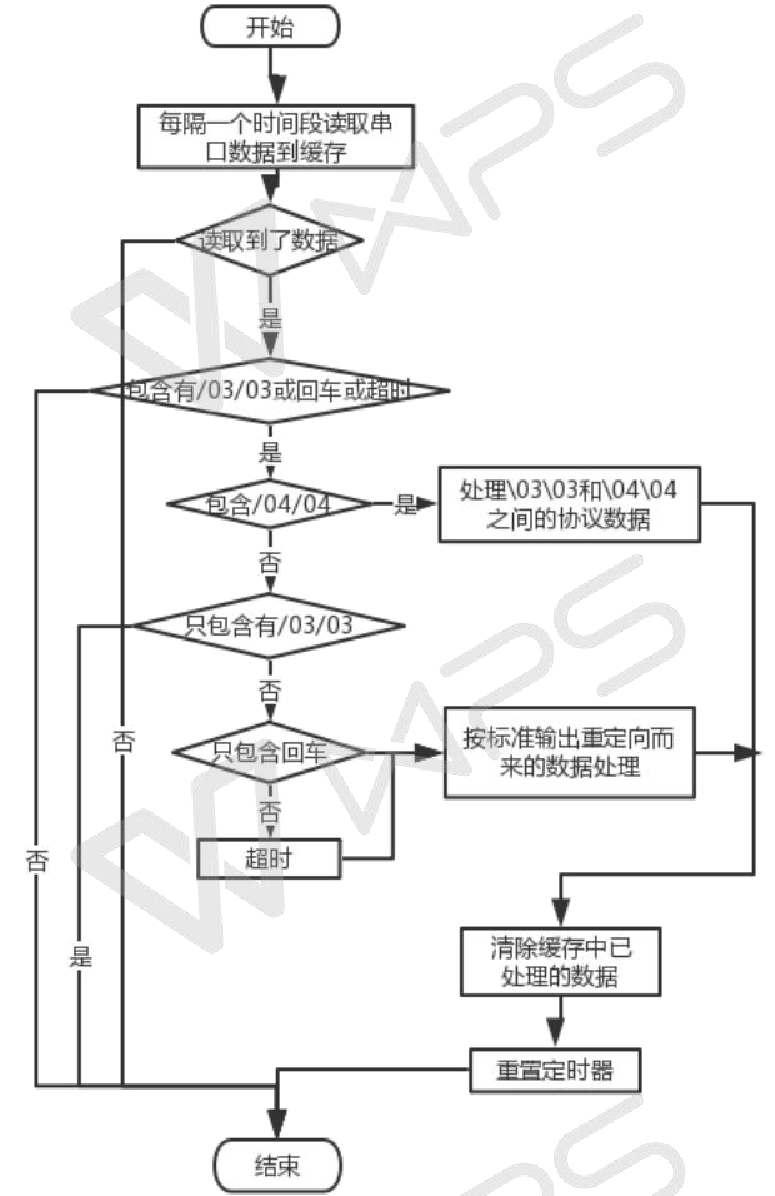
\includegraphics[width=.6\textwidth]{./graphics/LogTTYRead.pdf}
\caption{日志界面串口读取流程图}\label{fig:串口读取流程图}
\end{figure}

